%------------------------------------------------------------------------------
\chapter{Verification \& Validation}
\label{cha:validation}
%------------------------------------------------------------------------------

%------------------------------------------------------------------------------
\section{Overview}
%------------------------------------------------------------------------------

In order to show that the implementation of \neptune{} was successful, performing a verification and validation process is essential. In this context, 
verification will always be referred to comparing a method to another comparable one. In contrast, validation means that the results are compared to a \textit{truth}.

A validation process was set up for the state vector propagation, using freely available \gls{acr:poe} data for distinct satellites. The selected satellites 
are:
\begin{itemize}
 \item Jason-1: Oceanography satellite. 
 \item \acrshort{acr:gps}: 32 satellites of the \gls{acr:gps} constellation
 \item \acrshort{acr:ers}-1 and \acrshort{acr:ers}-2: Earth observation satellites
 \item \acrshort{acr:icesat}: Earth observation satellite
\end{itemize}

The validation process was performed in two steps. The first step consists of using a \gls{acr:poe} of the satellite under consideration as the initial state 
vector for the numerical propagation in \neptune{}. The second step consists of taking multiple \gls{acr:poe}s and assume them to be observations in order to 
perform a differential correction to find an initial state vector, which is expected to provide more accurate results. The following settings were used for 
\neptune{}:
\begin{itemize}
 \item Cannon-ball model for each satellite
 \item \acrshort{acr:egm}96, \num{70}$\times$\num{70} geopotential
 \item \gls{acr:eop}
 \item \acrshort{acr:nrl}\acrshort{acr:msis}E-00 atmosphere model
 \item Lunisolar gravitational perturbations
 \item Solar radiation pressure
 \item Solid Earth and ocean tides
 \item Earth radiation pressure
\end{itemize}

Alternatively, the state vector propagation can also be verified against another validated numerical integration tool. The main advantage here would be that all relevant orbit regions can be analysed, while using \glspl{acr:poe} is only possible for distinct orbits.

For the propagation of the covariance matrix propagation and the noise matrix evaluation a \gls{acr:mc} approach was used for the verification of the routines 
as a validation was not possible due to a lack of available data.

\section{State vector propagation validation}

%\begin{itemize}
% \item Post-processing often achieves accuracies of 2-10 cm radial position \cite{vallado2007}
% \item \gls{acr:tle} achieves km-level accuracy, can be at about 400 m, or even 50-100 m in post processing using numerical methods \cite{vallado2007}
% \item First possibility: Take single state vector from a \gls{acr:poe} and propagate without modification, as \gls{acr:poe} is assumed to be within an 
%accuracy of 2-10 cm (radial position).
% \item Second possibility: Slightly perturb satellite state (1 m) and compare against \gls{acr:poe}
% \item Propagation span shall be about 7-14 days, which is a typical span for operational decisions.
% \item In the drag regime:
% \item Optical properties, e.g. for TOPEX, LAGEOS, etc. can be obtained via \cite{knocke1989}.
% \item Credit to University of Texas \gls{acr:csr}
% \end{itemize}

% \subsection{Laser Geodynamics Satellites (LAGEOS)}
% \gls{acr:lageos}
%  \begin{itemize}
%   \item Promising candidate for small perturbing forces (SRP, ERP, Tides) due to simple geometry and low level of drag
%   \item Satellite properties in \cite{knocke1989}, p.43
%  \end{itemize}

\subsection{Jason-1}

The oceanography mission Jason-1 was launched in December 2001 as a successor to the TOPEX/Poseidon mission. With an initial mass of \SI{500}{\kilogram} it reached its 
first orbit about \SIrange{10}{15}{\kilo\metre} below the target orbit of TOPEX/Poseidon at \SI{1337}{\kilo\metre} \cite{nasaJason2014}. It then moved to the same orbit with an along-track 
separation to TOPEX/Poseidon of about \SI{500}{\kilo\metre}. It is thus reasonable to assume that the mass of Jason-1 was lower than \SI{500}{\kilogram} after it reached its final orbit. 
In \cite{vallado2007} the mass was set to \SI{475}{\kilogram}. The other required satellite parameters, which were used in the propagation with \neptune{}, are shown in 
\tab{tab:val-jason-data}.
\begin{table}[h!]
 \centering
 \caption{Satellite parameters used for Jason-1.\label{tab:val-jason-data}}
 \begin{tabular}{lS}
  \toprule
  \textbf{Parameter} & \textbf{Value} \\
  \cmidrule{1-2}
  Mass / \si{\kilogram}                         & 475.0 \\
  Cross-section / \si{\metre\squared}  & 10.0 \\
  Drag coefficient          & 2.2 \\
  \acrshort{acr:srp} coefficient & 1.2 \\
  \bottomrule
 \end{tabular}
\end{table}
While the satellite mass, drag coefficient and \gls{acr:srp} coefficient were equal to the values used in \cite{vallado2007}, for the cross-section a value of 
\SI{10.0}{\metre\squared} was estimated, based on the fact that the area of the solar panels is about \SI{9.5}{\metre\squared} and the box-shaped satellite has dimensions of 
\SI{954}{\milli\metre}$\times$\SI{954}{\milli\metre}$\times$\SI{2218}{\milli\metre}\footnote{\url{http://www.eoportal.org/directory/pres_Jason1AltimetryMission.html}, accessed on 2014-03-03.}.
 
The \gls{acr:poe} data was obtained from the \acrshort{acr:legos}-\acrshort{acr:cls} via the \gls{acr:ids} 
website\footnote{\url{http://ids-doris.org/welcome.html}, accessed on 2014-03-03.} in the \gls{acr:sp3} format for a period between March 20, 2002 and April 21, 
2002. That period was also used as the propagation span within \neptune{}.

The results for a 24-day propagation starting on March 24, 2002, are shown in \fig{fig:val-jas-01} \todo[TikZ conversion]{Provide Tikz image instead of GNUplot png}.
\begin{figure}[!h]
 \centering
 %%plot 'valjas_1_000.rad' u ($1-52357.0):10 w l lw 2 lt rgb 'green' title 'Cross-track', \
%     'valjas_1_000.rad' u ($1-52357.0):9  w l lw 2 lt rgb 'red'   title 'Along-track', \
%     'valjas_1_000.rad' u ($1-52357.0):8  w l lw 2 lt rgb 'blue'  title 'Radial'

\begin{tikzpicture}[scale=1]

  \begin{axis}[
      height=0.6\textwidth,
      width=0.8\textwidth,
      xlabel = {Day since March 4, 2002},
      ylabel = {Error/km},
      y tick label style={
       /pgf/number format/.cd,
           fixed,
           fixed zerofill,
           precision=1,
       /tikz/.cd
      },
      xmin   = 0,
      xmax   = 24,
      %clip=false,
      %restrict x to domain=23:25,
      %x coord trafo/.code={\pgfmathparse{#1-5.0}\pgfmathresult} % x-offset MJD
      ymin   = -0.2,
      ymax   = 1.8,
      %xtick  = {250,300,...,600},
      ytick  = {-0.2,0,0.2,...,1.8},
      %minor x tick num={1},
      %minor y tick num={3},
      scaled ticks = true,
      ymajorgrids,
      %yminorgrids,
      xmajorgrids,
      %xminorgrids,
      legend entries={Along-track, Cross-track, Radial} ,
      legend style={at={(0.02,0.98)}, anchor=north west},
      legend cell align = left
  ]
    \addplot[red, thick, smooth]          table {06-Validation/data/valjas_1_along2.out};
    \addplot[green, thick, smooth]        table {06-Validation/data/valjas_1_cross2.out};
    \addplot[blue, thick, smooth]         table {06-Validation/data/valjas_1_radial2.out};
    
  \end{axis}
  
\end{tikzpicture}
 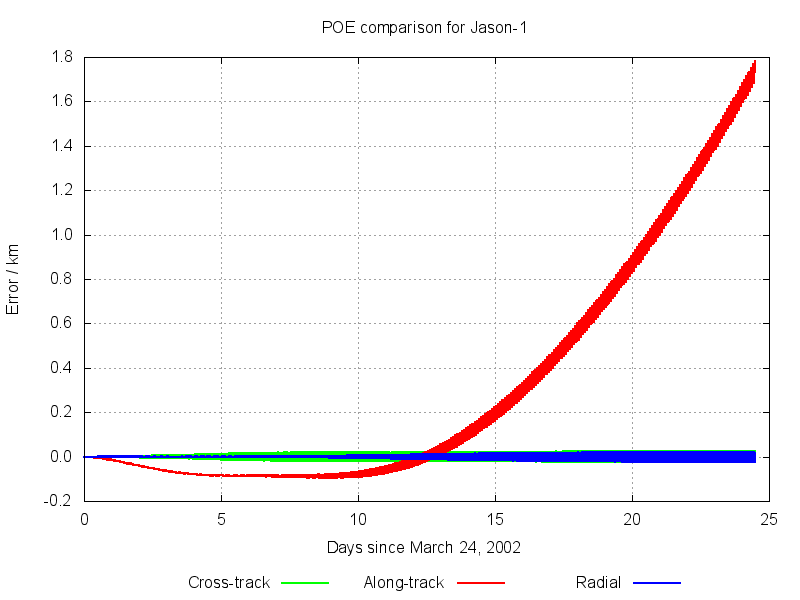
\includegraphics[width=0.85\textwidth]{val_jas_01.png}
 \caption{Comparison results for Jason-1.\label{fig:val-jas-01}}
\end{figure}
It can be seen that the error in the along-track component amounts to about one kilometre after three weeks of propagation.

A closer look at a smaller time interval of one day is shown in \fig{fig:val-jas-02} \todo[TikZ conversion]{Provide Tikz image instead of GNUplot png}.
\begin{figure}[!h]
 \centering
 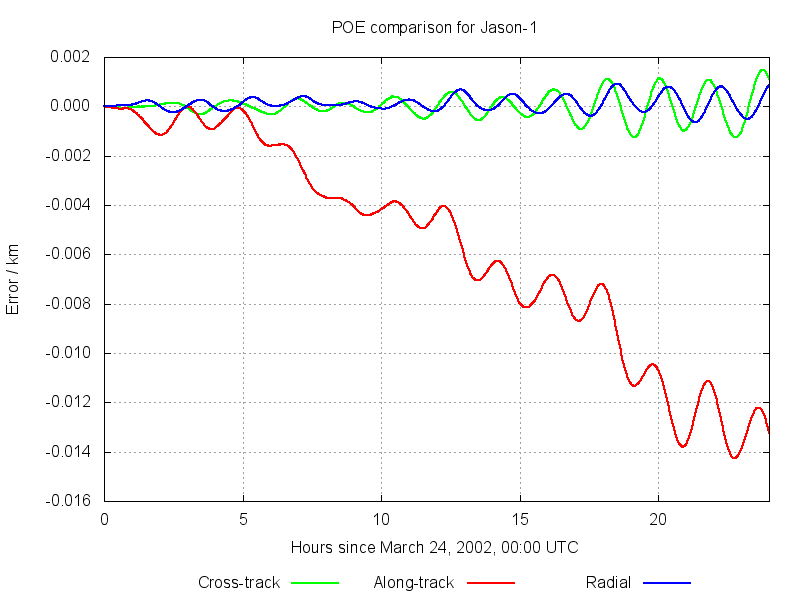
\includegraphics[width=0.85\textwidth]{val_jas_02.png}
 \caption{Comparing results for Jason-1 for a one-day propagation.\label{fig:val-jas-02}}
\end{figure}
The error in the along-track component is at about \num{14} metres after one day. The quite irregular looking evolution of the along-track error is basically due to 
the Solar and Earth radiation pressure contributions, as Jason-1 was modelled as a spherically shaped object. This becomes more obvious, when looking at the 
error evolution after switching these two perturbations off subsequently. In \fig{fig:val-jas-03} \todo[TikZ conversion]{Provide Tikz image instead of GNUplot png} the Earth radiation pressure (short-wave albedo and long-wave 
infrared) was switched off.
\begin{figure}[!h]
 \centering
 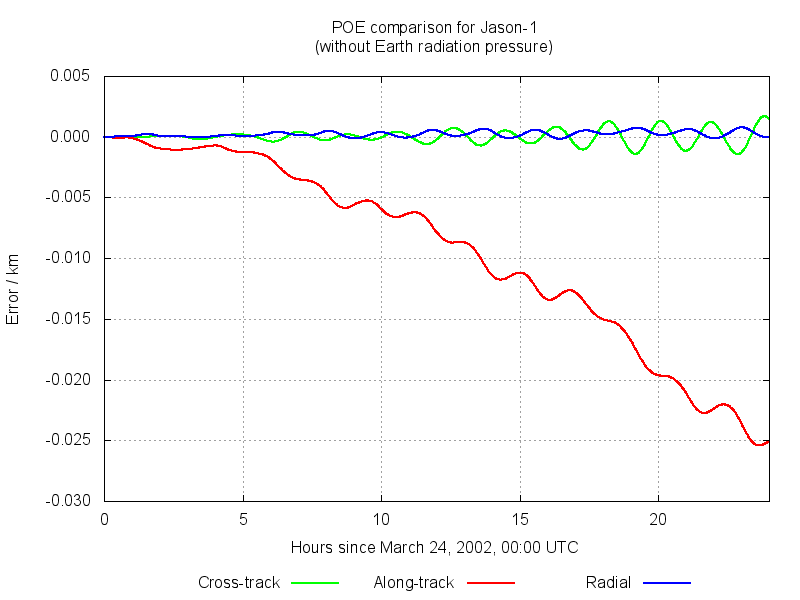
\includegraphics[width=0.85\textwidth]{val_jas_03.png}
 \caption{Comparing results for Jason-1 for a one-day propagation without Earth radiation pressure.\label{fig:val-jas-03}}
\end{figure}
The error increases to about 25 metres after one day, when Earth's radiation pressure is not considered. When solar radiation pressure is also switched off, 
the along-track error increases to about 65 metres after one day as shown in \fig{fig:val-jas-04}.
\begin{figure}[!h]
 \centering
 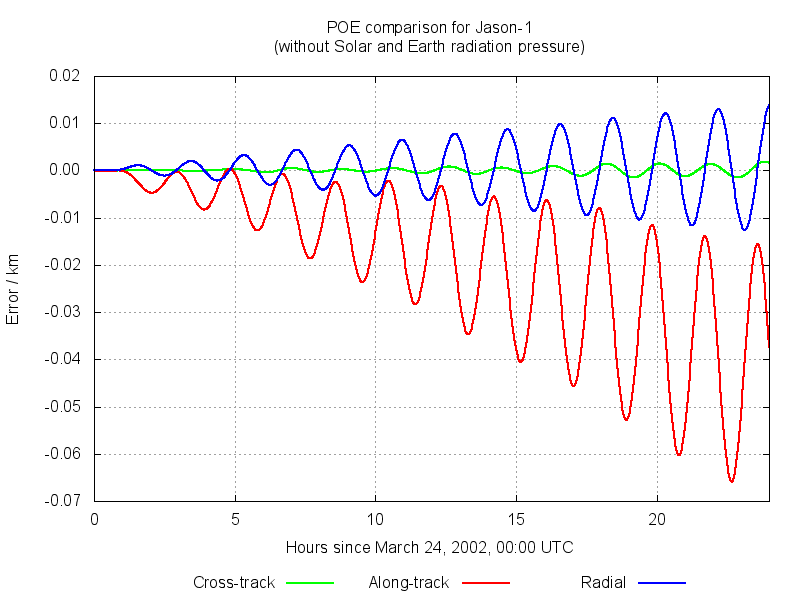
\includegraphics[width=0.85\textwidth]{val_jas_04.png}
 \caption{Comparing results for Jason-1 for a one-day propagation without Solar and Earth radiation pressure.\label{fig:val-jas-04}}
\end{figure}

\subsection{Global Positioning System (GPS)}

The validation using \gls{acr:gps} precision ephemerides is based on data available from the \gls{acr:nga} website \cite{nga2013}. The data was downloaded from 
the \gls{acr:nga} \acrshort{acr:ftp} server\footnote{\url{ftp://ftp.nga.mil/pub2/gps/pedata/}} for the year 2013. 

For the validation it is essential to use a time span free of any orbital maneuvers for the satellites under consideration. Therefore the so-called 
\gls{acr:nanu} messages were used, which are provided by the U.S. Coast Guard Navigation Center\footnote{\url{http://navcen.uscg.gov/?pageName=gpsAlmanacs}} 
for the \gls{acr:gps} satellites, containing information on which satellite is expected to have forecast outages for which period of time. A good 
overview on the available \gls{acr:nanu} messages for an individual year can also be found at the Celestrak website \cite{celestrak-nanu-2014}.

Extracting all the required information from the \gls{acr:nanu}s for 2013, one gets a good picture of which time frames are adequate to perform a validation 
for the complete \gls{acr:gps} constellation. The result of such an analysis is shown in \fig{fig:val-gps-nanu-2013}.
\begin{figure}[h!]
 \centering
 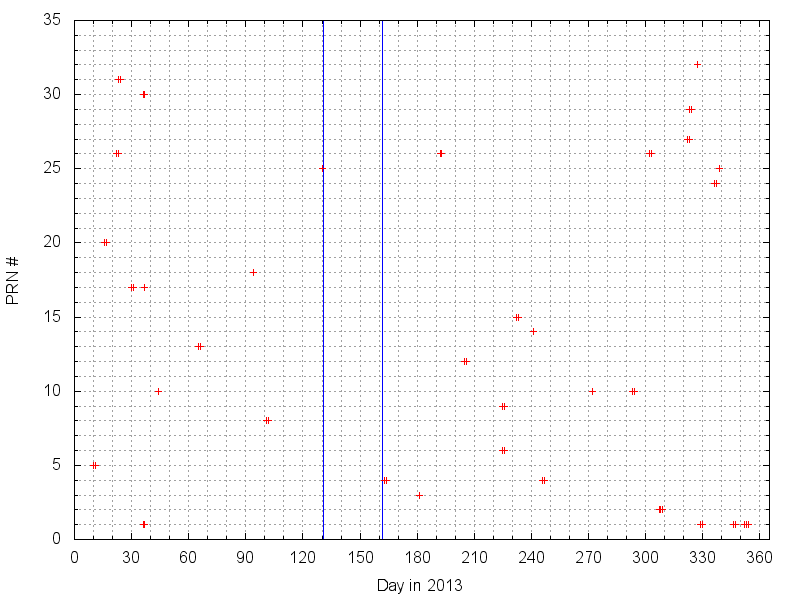
\includegraphics[width=0.85\textwidth]{nanu_summary_2013.png}
 \caption{Unusable ephemerides for all GPS satellites in 2013. The time span between the two vertical lines (blue) can 
be used in the validation analysis.\label{fig:val-gps-nanu-2013}}
\end{figure}
It can be seen that there is a window of approximately three weeks between day 131 and day 162 as indicated by the vertical blue lines, corresponding to a time frame of one month between May 11, 2013 and June 11, 2013.

The currently operational \gls{acr:gps} constellation consists of 32 satellites (as of February 2014) from the \textit{Block II} 
generation only \cite{gps2014} with satellites of the 
\textit{Block III} generation being under production. For the operational satellites a further subdivision is possible \cite{navcen2014}:
\begin{itemize}
 \item \textbf{Block IIA:} 8 operational, second generation, ``Advanced''
 \item \textbf{Block IIR:} 12 operational, ``Replenishment''
 \item \textbf{Block IIR(M):} 8 operational, ``Modernized''
 \item \textbf{Block IIF:} 4 operational, ``Follow-on''
\end{itemize}

It is important to consider the different types of Block II satellites in order to have an appropriate estimate of the cross-sectional area and the mass. In \tab{tab:val-gps-sats} the currently operational satellites are shown together with their \gls{acr:prn} code, the dimensions\footnote{Width across solar panels} 
and the mass, which were also used 
for the validation.
\begin{table}[h!]
 \centering
 \caption{Current GPS constellation as of February 26, 2014 \citep{navcen2014, about.com2014}.\label{tab:val-gps-sats}}
 \begin{tabular}{lp{5cm}lS}
 \toprule
  \textbf{Type} & \textbf{PRNs} & \textbf{Dim. W$\times$D$\times$H / \si{\milli\metre}} & \textbf{Mass / \si{\kilogram}} \\
  \cmidrule{1-4}
  Block IIA    & 3,  4,  6,  8,  9, 10, 26, 32      &        5300 $\times$ 3400 $\times$ 3400 & 840 \\
  Block IIR    & 2, 11, 13, 14, 16, 18-23, 28       & 11\ 400 $\times$ 1956 $\times$ 2210 & 1127 \\
  Block IIR(M) & 5,  7, 12, 15, 17, 29, 30$^*$, 31  & 11\ 400 $\times$ 1956 $\times$ 2210 & 1127 \\
  Block IIF    & 1, 24, 25, 27$^{**}$               & 11\ 820 $\times$ 2032 $\times$ 2235 & 1465 \\
  \bottomrule
  \multicolumn{1}{r}{\footnotesize $^*$}    & \multicolumn{3}{l}{\footnotesize PRN30 was launched on Feb 21, 2014 \citepalias{nanu2014018} and is not considered in 
the validation.} \\
  \multicolumn{1}{r}{\footnotesize $^{**}$} & \multicolumn{3}{p{12cm}}{\footnotesize PRN27 was launched on May 15, 2013 \citepalias{nanu2013031} and is not considered 
in the validation.} \\   
 \end{tabular}
\end{table}
From the 32 active satellites in the constellation, for the selected validation time frame only 30 satellites may be used. \acrshort{acr:prn}27 was launched 
within that time span on May 15, 2013 \citepalias{nanu2013031} and was fully operational from June 21, 2013 \citepalias{nanu2013035}, so that it could not be used in the validation. Also, \acrshort{acr:prn}30 was launched on February 21, 2014 \citepalias{nanu2014018} and is currently in its testing phase.

For the simulations by \neptune{} it is required to estimate the cross-section of the GPS satellites based on the dimensions as specified in different sources for the different types of Block II objects. As for satellites in the GPS constellation the effective cross-section relative to the Sun's direction is significant, it was assumed that the full area of the solar panels contributes to the total cross-section. For the main body, the average of the three different surfaces of the rectangular cuboid (box) was computed. The total cross-section as well as the drag and \gls{acr:srp} parameter, which were used in the validation, are shown in \tab{tab:val-gps-sim-data}.
\begin{table}[h!]
 \centering
 \caption{Cross-section, \gls{sym:c_d} and \gls{sym:c_srp} of \acrshort{acr:gps} satellites used in the validation.\label{tab:val-gps-sim-data}}
 \begin{tabular}{lSSS}
  \toprule
  	\textbf{Type} & \textbf{Cross-section / \si{\metre\squared}} & \textbf{\gls{sym:c_d}} & \textbf{\gls{sym:c_srp}} \\
  \cmidrule{1-4}
  Block IIA       &     18.02 & 2.2 & 1.3\\
  Block IIR      &     22.63 & 2.2 & 1.3\\
  Block IIR(M) &     22.63 & 2.2 & 1.3\\
  Block IIF       &     24.29 & 2.2 & 1.3\\
  \bottomrule
 \end{tabular}
\end{table}

The \gls{acr:poe} data for \gls{acr:gps} satellites is obtained in the SP3 format \citep{remondi1989}, where the cartesian state vectors in five minute intervals are given in the \acrshort{acr:wgs}84 frame. In \neptune{} the \gls{acr:itrf} is used, however, \acrshort{acr:wgs}84 is closely aligned to the 
\gls{acr:itrf} \citep{tapley2004} so that no coordinate transformation was required at this point. Instead, the ephemerides were converted to \gls{acr:gcrf} in order to be compared with the trajectory as propagated by \neptune{}. Some exemplary results are shown in the following.
\begin{figure}[!h]
 \centering
 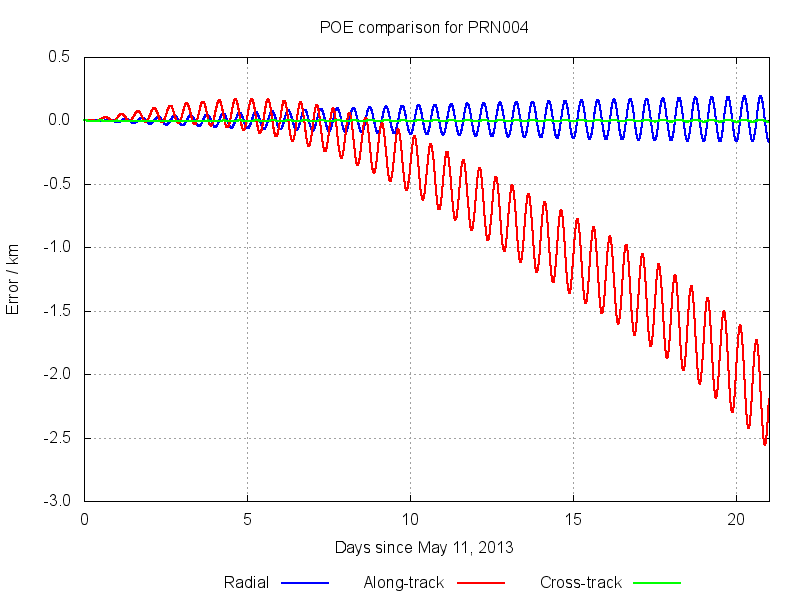
\includegraphics[width=0.85\textwidth]{val_gps_prn04.png}
 \caption{Comparison results for PRN04.\label{fig:val-gps-prn04}}
\end{figure}

\begin{figure}[!h]
 \centering
 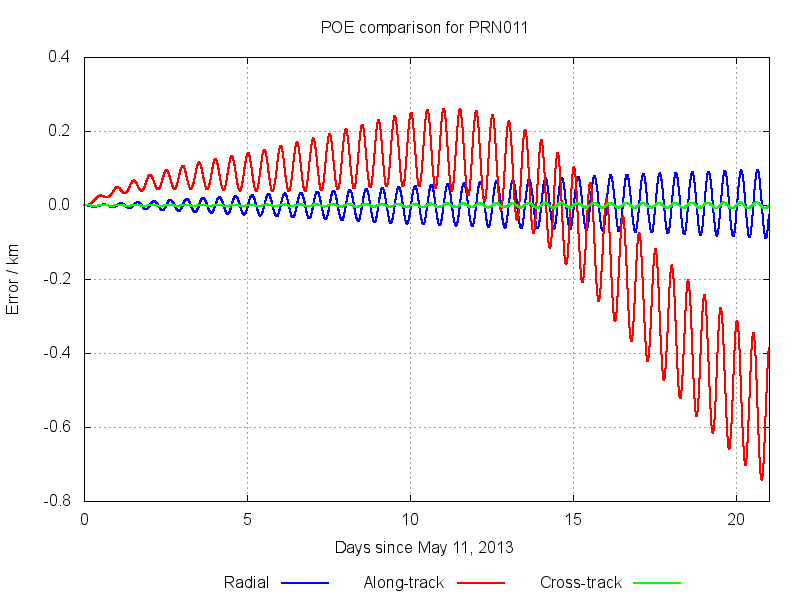
\includegraphics[width=0.85\textwidth]{val_gps_prn11.png}
 \caption{Comparison results for PRN11.\label{fig:val-gps-prn11}}
\end{figure}

In \fig{fig:val-gps-prn04} the result for \acrshort{acr:prn}04 is shown. The error in the along-track component is about \SI{2.5}{\kilo\metre} after 21 days. However, there were also examples, where the error was significantly lower, as for example in the case of \acrshort{acr:prn}11, where the along-track error is at about \SI{700}{\metre} after the same period of 21 days. It can also be seen that the radial error for \acrshort{acr:prn}11 is lower than for \acrshort{acr:prn}04, which, of 
course, correlates with the evolution of the along-track component.

A third example is shown in \fig{fig:val-gps-prn09} for \acrshort{acr:prn}09. Here, the along-track error increases to about \SI{3.5}{\kilo\metre} after 21 days, while the radial error is almost at \SI{500}{\metre}. 

\begin{figure}[!h]
 \centering
 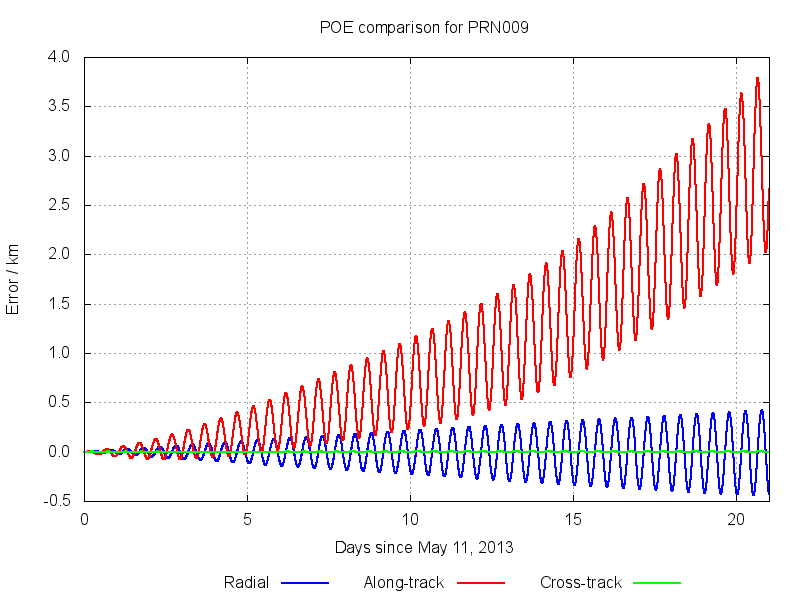
\includegraphics[width=0.85\textwidth]{val_gps_prn09.png}
 \caption{Comparison results for PRN09.\label{fig:val-gps-prn09}}
\end{figure}

The errors in all examples are showing a fluctuation with a period of one orbit, which is typical for a model misalignment. This was expected, as the first \gls{acr:poe} was selected to be the initial state for \neptune{} which then propagates with another model as compared to the one used for the \gls{acr:poe} generation.

\subsection{European Remote Sensing Satellites (ERS-1 and -2)}

The first mission \acrshort{acr:ers}-1 was launched on July 17, 1991 and was accompanied by \acrshort{acr:ers}-2 on April 21, 1995 with both objects put into a sun-synchronous orbit between \SIrange{782}{785}{\kilo\metre}
\footnote{\url{https://earth.esa.int/web/guest/missions/esa-operational-eo-missions/ers/satellite}\label{foot:esa}}. From \acrshort{acr:esa}'s 
website$^{\ref{foot:esa}}$ an initial estimate for the satellite parameters was derived, shown in \tab{tab:val-ers-data}. Missing parameters, being the drag and \gls{acr:srp} coefficients, were taken from \cite{vallado2007}.
\begin{table}[h!]
 \centering
 \caption{Satellite parameters used for \gls{acr:ers}-1 and \gls{acr:ers}-2.\label{tab:val-ers-data}}
 \begin{tabular}{lS}
 \toprule
  	\textbf{Parameter} & \textbf{Value} \\
  \cmidrule{1-2}
  Mass / \si{\kilogram}                 & 2300 \\
  Cross-section / \si{\metre\squared}     & 35.0 \\
  Drag coefficient          & 2.5 \\
  \acrshort{acr:srp} coefficient & 1.0 \\
  \bottomrule
 \end{tabular}
\end{table}

For \acrshort{acr:ers}-1 the first propagation was performed starting on August 4, 1991. The result is shown in \fig{fig:val-ers1-01}.
\begin{figure}[!h]
 \centering
 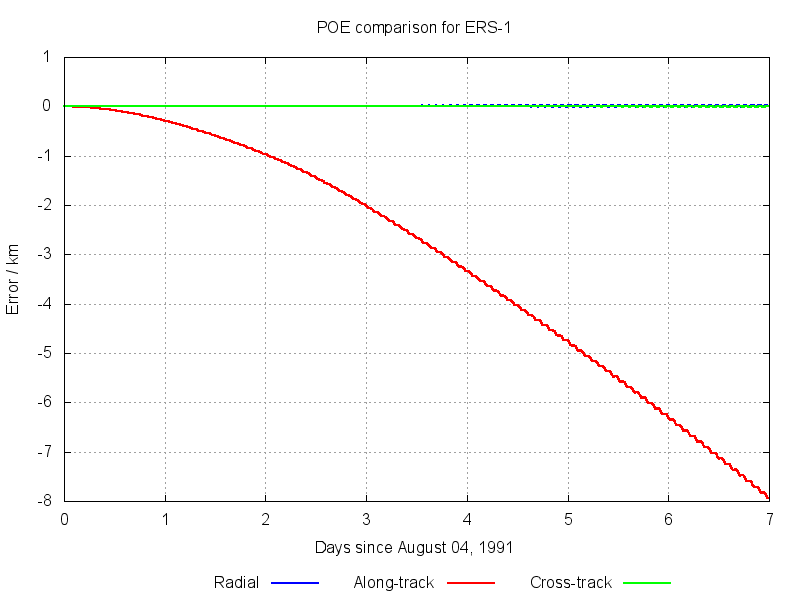
\includegraphics[width=0.85\textwidth]{valers1_1.png}
 \caption{Comparison results for ERS-1 for a one-week propagation.\label{fig:val-ers1-01}}
\end{figure}
After a one-week propagation, the accumulated error in the along-track component is about eight kilometers. 

For a shorter time frame of about six hours starting from the initial epoch, the error is shown in \fig{fig:val-ers1-02}.
\begin{figure}[!h]
 \centering
 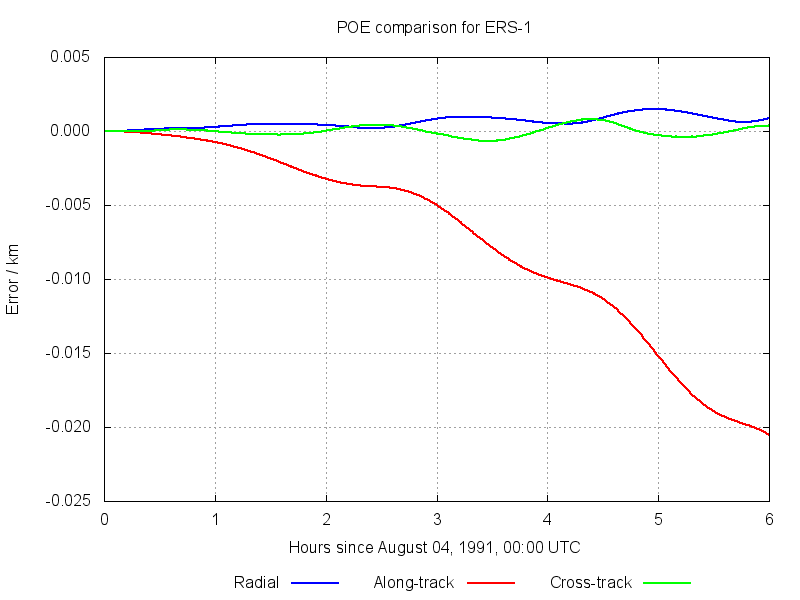
\includegraphics[width=0.85\textwidth]{valers1_2.png}
 \caption{Comparison results for ERS-1 for a six-hour propagation.\label{fig:val-ers1-02}}
\end{figure}
The radial error increases after each revolution by about one meter which leads to the build-up in along-track error. This indicates, as the radial error is positive, that \acrshort{acr:ers}-1 was decaying faster than the propagated orbit of \neptune{}, as in general the error was computed via:
\begin{equation}
  \Delta \vec{r} = \vec{r}_{NEPTUNE} - \vec{r}_{ERS}
\end{equation}
While the considered epoch for \acrshort{acr:ers}-1 was within a period of increased solar activity, for \acrshort{acr:ers}-2 it was looked at whether the situation changes during low solar activity. Therefore, the initial epoch was selected to be at September 8, 1995. Also, the cross-section was adapted to \SI{11}{\metre\squared} and the mass set to \SI{2200}{\kilogram} to make the results comparable to the ones obtained in \cite{vallado2007}. The errors for a propagation span of one week are shown 
in \fig{fig:val-ers2-01}.
\begin{figure}[!h]
 \centering
 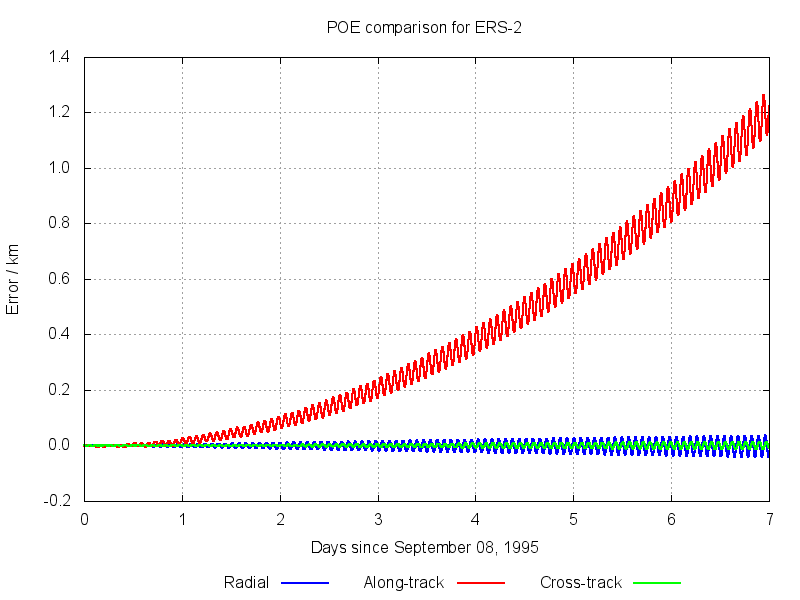
\includegraphics[width=0.85\textwidth]{valers2_1.png}
 \caption{Comparison results for ERS-2 for a one-week propagation.\label{fig:val-ers2-01}}
\end{figure}
It can be seen that the resulting error after seven days in the along-track component is about \SI{1.2}{\kilo\metre}. It was at about \SI{10}{\kilo\metre} when using the satellite parameters as given in \tab{tab:val-ers-data} which were used for \acrshort{acr:ers}-1. However, using another set of parameters for \acrshort{acr:ers}-1, for example as used for \acrshort{acr:ers}-2 in \fig{fig:val-ers2-01}, did not provide better results. It can thus be argued that solar activity has a significant influence on the prediction accuracy, even if the solar and geomagnetic activity data used in the simulation was observed data for the considered 
propagation spans. 

\subsection{Ice, Cloud, and land Elevation Satellite (ICESat)}

\gls{acr:icesat} was part of \acrshort{acr:nasa}'s Earth observation system between 2003 and 2009 and its mission was to measure the ice sheet mass balance, cloud 
and aerosol heights, as well as perform land topography and analyse vegetation characteristics \footnote{\url{http://icesat.gsfc.nasa.gov/}}. The 
\gls{acr:poe}s for \gls{acr:icesat} were obtained from the \acrshort{acr:ftp} server of the \gls{acr:csr} at the University of Texas \citep{csr2014} for a time frame between September 24, 2003 and November 18, 2003.

As \gls{acr:icesat} was operated in an orbit at about \SI{600}{\kilo\metre} altitude, atmospheric drag was providing a significant contribution to the orbital evolution. 
Therefore, it is essential to have a good estimate of the ballistic parameter. In a similar study by \cite{vallado2007}, an initial mass of \SI{970}{\kilogram} was reduced to about \SI{950}{\kilogram}, assuming that some maneuvering fuel had been spent, to be used in the simulation for February 2003.

For the \neptune{} validation and the time frame between September and November 2013, a value of \SI{950}{\kilogram} was used as a starting value. Also, in 
\cite{vallado2007} further required values are given, which were used in the following analyses and are shown in \tab{tab:val-ice-data}.
\begin{table}[h!]
 \centering
 \caption{Satellite parameters used for \gls{acr:icesat}.\label{tab:val-ice-data}}
 \begin{tabular}{lS}
 \toprule
	\textbf{Parameter} & \textbf{Value} \\
  \cmidrule{1-2}
  Cross-section / \si{\metre\squared}   & 2.0 \\
  Drag coefficient          & 2.2 \\
  \acrshort{acr:srp} coefficient & 1.0 \\
  \bottomrule
 \end{tabular}
\end{table}

The first analysis was done for a propagation span of a few days, starting at September 25, 2003, 21:00 \acrshort{acr:utc}. The results can be seen in 
\fig{fig:val-ice-01}.
\begin{figure}[!h]
 \centering
 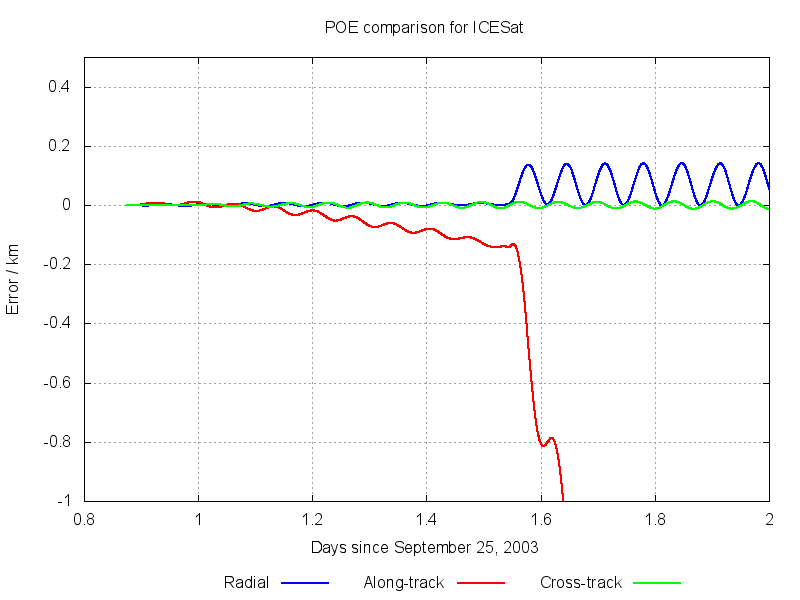
\includegraphics[width=0.85\textwidth]{valice01.png}
 \caption{Comparison results for ICESat showing a maneuver on September 26, 2003.\label{fig:val-ice-01}}
\end{figure}
While initially the errors in all three components are in the order of magnitude between \SIrange{10}{100}{\metre} with the along-track component showing an expected drift, on September 26, 2003 a maneuver can be identified, which manifests itself through a sudden change in slope for the along-track error and a sudden increase in the 
mean radial error. 
For the next analysis, the initial epoch was set to September 27, 2003, 21:00 \gls{acr:utc}, which is about one and a half days beyond the previous maneuver. 
As can be seen in \fig{fig:val-ice-02}, for a period free of maneuvers, the along-track error amounts to about one kilometer after about three days of 
propagation.
\begin{figure}[!h]
 \centering
 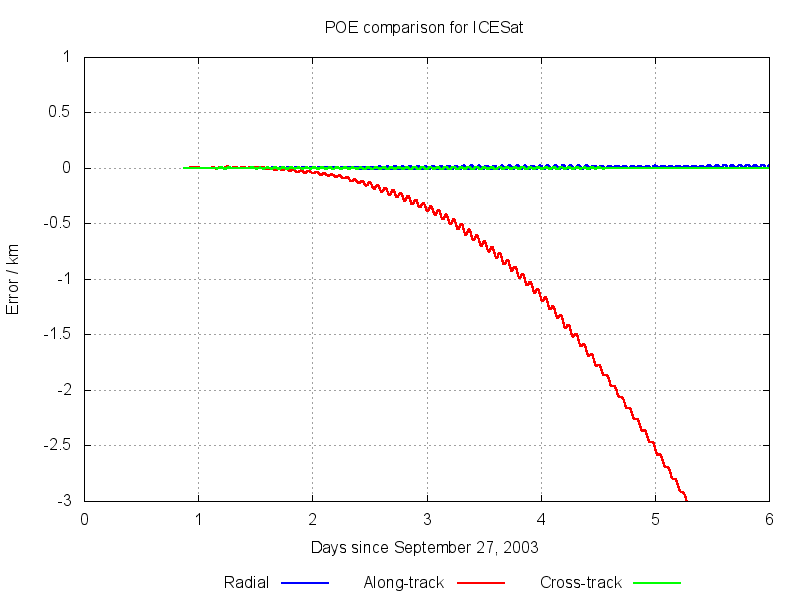
\includegraphics[width=0.85\textwidth]{valice02.png}
 \caption{Comparison results for ICESat for about four days after September 27, 2003, 21:00 UTC.\label{fig:val-ice-02}}
\end{figure}
This behaviour is expected in the presence of atmospheric drag, which becomes even more obvious when looking at the radial component alone as shown in 
\fig{fig:val-ice-03}.
\begin{figure}[!h]
 \centering
 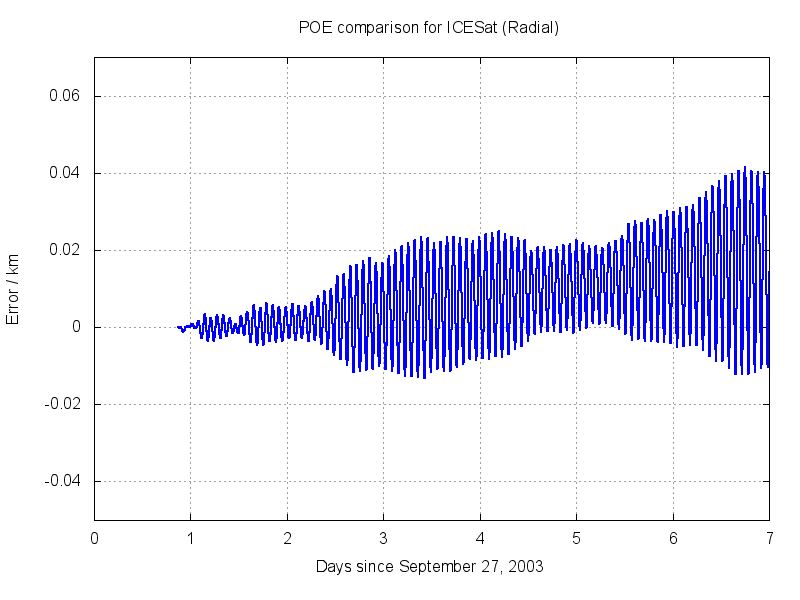
\includegraphics[width=0.85\textwidth]{valice03.png}
 \caption{Comparison results for ICESat: Radial error after September 27, 2003, 21:00 UTC.\label{fig:val-ice-03}}
\end{figure}
Here, the radial error shows a drift which means that \gls{acr:icesat} was descending with a faster rate than what \neptune{} predicted, as the error, in 
general, was computed by:
\begin{equation}
 \Delta \vec{r} = \vec{r}_{NEPTUNE} - \vec{r}_{ICESat}
\end{equation}
A faster descent would suggest that \gls{acr:icesat} had a lower mass (or a higher cross-section) as was initially assumed. Due to the maneuver on September 
26, it could be possible that the mass after that maneuver was below \SI{950}{\kilogram}. This seems to be even more reasonable when considering the fact that the mass 
estimate is based on \cite{vallado2007}, where the analysis was done for February 2003, with a few possible additional maneuvers until September 2003. Therefore, another validation run was performed after decreasing the mass to \SI{900}{\kilogram} and the result is shown in \fig{fig:val-ice-04}.
\begin{figure}[!h]
 \centering
 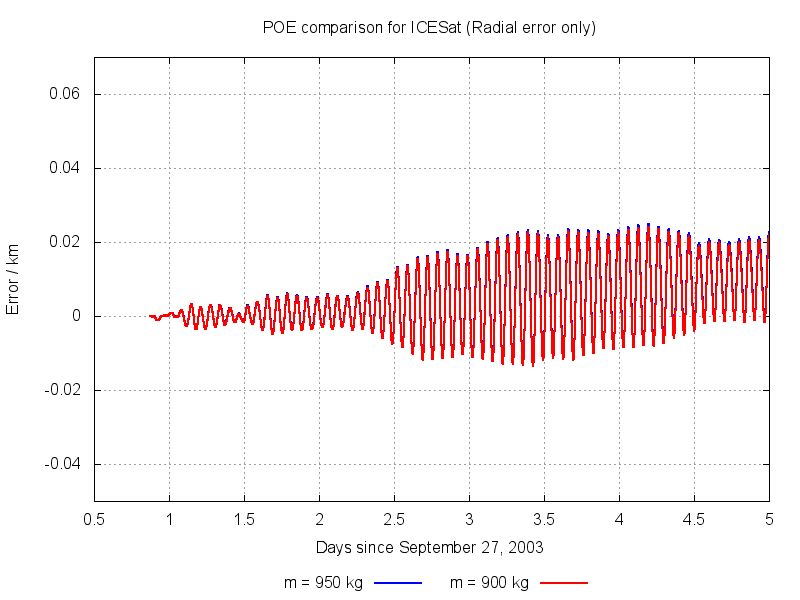
\includegraphics[width=0.85\textwidth]{valice04.png}
 \caption{Comparison results for ICESat: Radial error for a different initial mass.\label{fig:val-ice-04}}
\end{figure}
It can be seen that a reduced mass does not affect the result significantly. 

In \cite{vallado2007} it is mentioned that \gls{acr:icesat} may fly in a ``sailboat'' orientation, where the solar panels contribute most in velocity direction. A value of \SI{5.21}{\metre\squared} is given in \cite{vallado2007} together with an 
adapted drag coefficient of \gls{sym:c_d}=\num{2.52}. The result for this simulation is shown in \fig{fig:val-ice-05}.
\begin{figure}[!h]
 \centering
 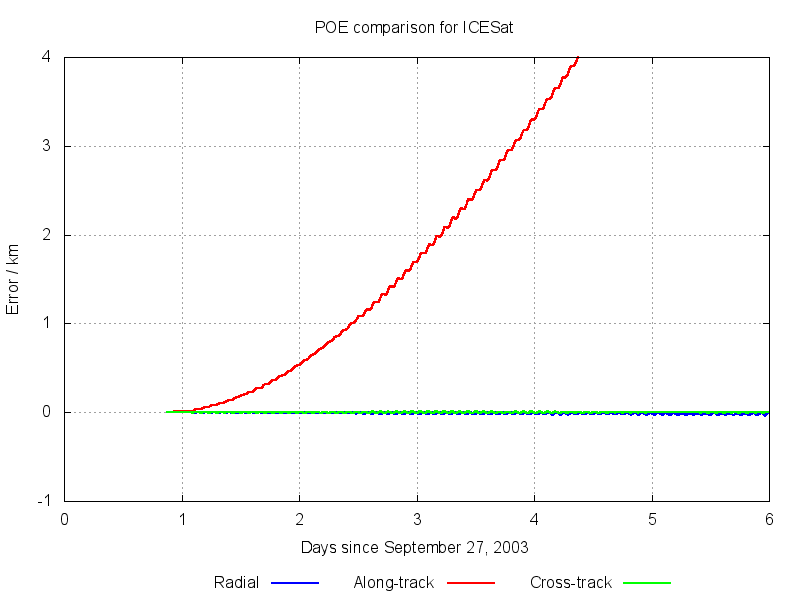
\includegraphics[width=0.85\textwidth]{valice05.png}
 \caption{Comparison results for ICESat: Error in ``sailboat'' orientation mode.\label{fig:val-ice-05}}
\end{figure}
It can be seen that the along-track error in this case is positive which means that the propagation by \neptune{} is trailed by \gls{acr:icesat} meaning that 
\neptune{} now results in predicting a too fast decay. As the error is at about one kilometer after two days - as compared to the same along-track error after 
three days in \fig{fig:val-ice-02} - a ``sailboat'' orientation seems unlikely for this period. However, an orientation somewhere in between the two analysed 
cases should provide a better solution, which is exemplarily shown in \fig{fig:val-ice-06} for a cross-section of \SI{3.0}{\metre\squared}.
\begin{figure}[!h]
 \centering
 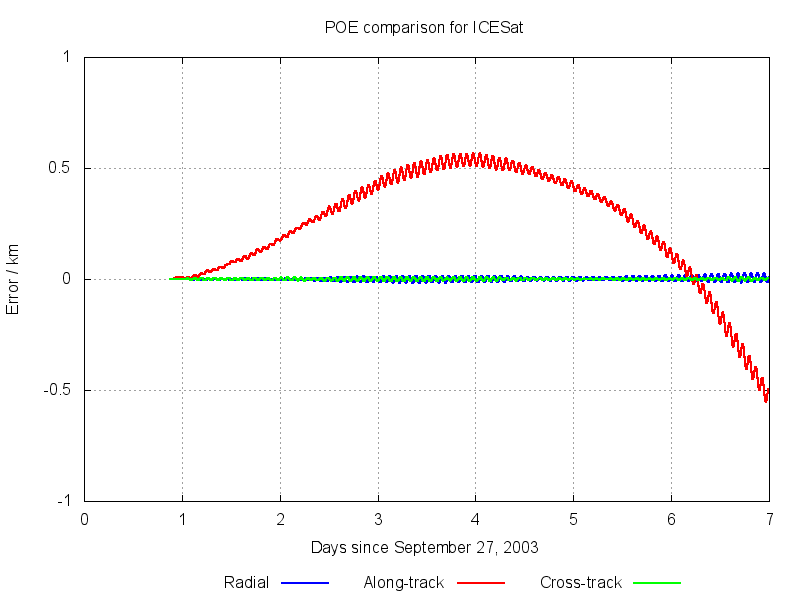
\includegraphics[width=0.85\textwidth]{valice06.png}
 \caption{Comparison results for ICESat: Error for a cross-section of \SI{3.0}{\metre\squared}.\label{fig:val-ice-06}}
\end{figure}

\section{Covariance matrix propagation verification}

The verification of the covariance matrix propagation in \neptune{} was done by a \gls{acr:mc} analysis. Therefore, a dedicated tool was developed: \cover{} (Covariance Verification). Its task, as shown in \fig{fig:val-cover-scheme}, is to receive the initial covariance matrix used by \neptune{} and to generate an object cloud representing the underlying statistics from the uncertainties in the state vector.
\begin{figure}[!h]
  \centering
  \setlength{\abovecaptionskip}{0.5cm}
     
  \begin{tikzpicture}[scale=0.7, transform shape, node distance=0.5cm, >=latex]
 
    \node (cover)     [redbox] 				{\textbf{COVER}};
    \node (input)     [bluebox, below =of cover]  	{Read input file: cover.inp};
    \node (inpfile)   [speicher, right=of input]  	{Input};
    \node (cloud)     [bluebox, below =of input]  	{Generate object cloud based on variance/covariance matrix};
    \node (loop_time) [branch, below=of cloud]		{\textbf{Loop:} Time};
    \node (time)      [bluebox, right=of loop_time]     {Increment time};
    \node (parent)    [bluebox, below=of time]          {Propagate parent's state and covariance};
    \node (loop_obj)  [branch, below=of parent]		{\textbf{Loop:} Objects};
    \node (objects)   [bluebox, below right=0.5cm and 1cm of loop_obj]      {Propagate object's state};
    \node (end1)      [branch, below=1cm of loop_obj]	{\textbf{End?}};
    
    \node (uvw)       [bluebox, below=of end1]       	{Convert states to UVW frame};
    \node (stats)     [bluebox, below=of uvw]        	{Process statistics};
    \node (output1)   [bluebox, below =of stats]     	{Write line to output: $<$RUNID$>$.cov};
    \node (output2)   [bluebox, below =of output1]   	{Write line to output: $<$RUNID$>$.prop.cov};
    \node (prop_file) [speicher, right=of output2]     	{Propagated covariance matrix};
    \node (cov_file)  [speicher, right=of output1]   	{Object cloud statistics};
    \node (end2)      [branch, below=13cm of loop_time]	{\textbf{End?}};
    \node (end)       [redbox, below=of end2]          	{\textbf{End}};


    \draw [->] (cover)     to (input);
    \draw [->] (inpfile)   to (input);
    \draw [->] (input)     to (cloud);
    \draw [->] (cloud)     to (loop_time);
    \draw [->] (loop_time) to (time);
    \draw [->] (time)      to (parent);
    \draw [->] (parent)    to (loop_obj);
    \draw [->] (loop_obj)  -| (objects);
    \draw [->] (end1)      to (loop_obj);
    \draw [->] (end1)      to (uvw);
    \draw [->] (uvw)       to (stats);
    \draw [->] (stats)     to (output1);
    \draw [->] (output1)   to (cov_file);
    \draw [->] (output1)   to (output2);
    \draw [->] (output2)   to (prop_file);
    \draw [->] (end2)      to (loop_time);
    \draw [->] (end2)      to (end);
% 
    \draw [->] (objects.south) |- (end1.east);
    \draw [->] (output2.south) |- (end2.east);

  \end{tikzpicture}
  \caption{Schematic overview of the \cover{} tool.}
  \label{fig:val-cover-scheme}
\end{figure}

As the radius and the velocity component errors present in the variance/covariance matrix are correlated, a Cholesky decomposition has to be performed. For the 
covariance matrix \gls{sym:P} the Cholesky decomposition is defined as:
\begin{equation}
 \gls{sym:P} = \gls{sym:L}\cdot\gls{sym:L}^T
\end{equation}
It is assumed that the initial errors in the state vector are normally distributed, so that random variables \gls{sym:Z} are computed according to a standard 
normal distribution:
\begin{equation}
 \gls{sym:Z} = \mathcal{N}\left(0,1\right)
\end{equation}
Then, for each object, the state vector can be sampled using six random numbers (for position and velocity), given via the vector $\gls{sym:z}_i = 
\left[\gls{sym:Z}_1,\ldots,\gls{sym:Z}_6\right]$ and the mean $\overline{\gls{sym:state}}$, which is the associated state vector:
\begin{equation}
 \gls{sym:state}_i = \gls{sym:L}\cdot\gls{sym:z}_i + \overline{\gls{sym:state}}
\end{equation}

For each generated object an individual \neptune{} propagation run for the sampled state vector to a certain reference epoch is performed. At this epoch the 
object cloud is processed to extract its statistics and form the covariance matrix for that point in time again. The result is then compared to the numerical 
integration of the covariance matrix as implemented in \neptune{}. 

The verification process of the covariance matrix propagation contained different scenarios with varying initial covariance matrix, as defined in the following 
list:
\begin{enumerate}
 \item Propagation of object cloud considering only the central body force.
 \item Scenario 1 + geopotential with order $\gls{sym:geo_n}=2$.
 \item Scenario 1 + geopotential with order $\gls{sym:geo_n}>2$.
 \item Scenario 1 + atmospheric drag
\end{enumerate}

\paragraph{Scenario 1: Central body force}

In the first scenario, only the central body force was used for the object cloud consisting of one parent object (identical to the state vector corresponding 
to the covariance matrix) and 499 generated objects according to the uncertainty in the state.

The first example for an initial radial error of \SI{1}{\metre}, and no error in the other components, is shown in \fig{fig:val-cov-scen1-01} for a circular orbit at \SI{300}{\kilo\metre} altitude and \ang{50;;} inclination.
\begin{figure}[h!]
  \centering
  \subfigure[Position]{\label{fig:val-cov-scen1-01a} 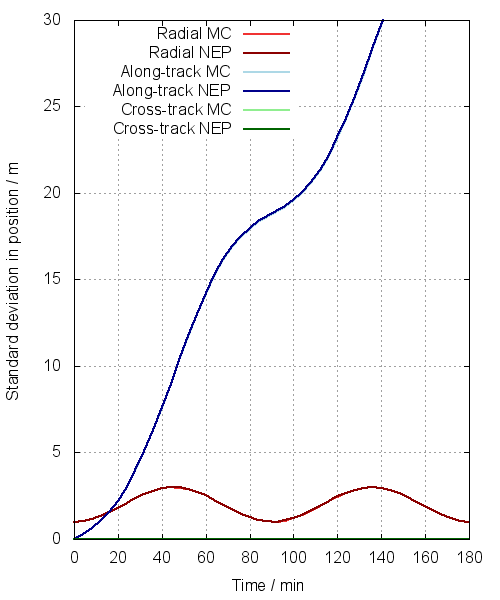
\includegraphics[width=0.4\textwidth]{2B_1_rad.png}}
  \hspace{1cm}
  \subfigure[Velocity]{\label{fig:val-cov-scen1-01b} 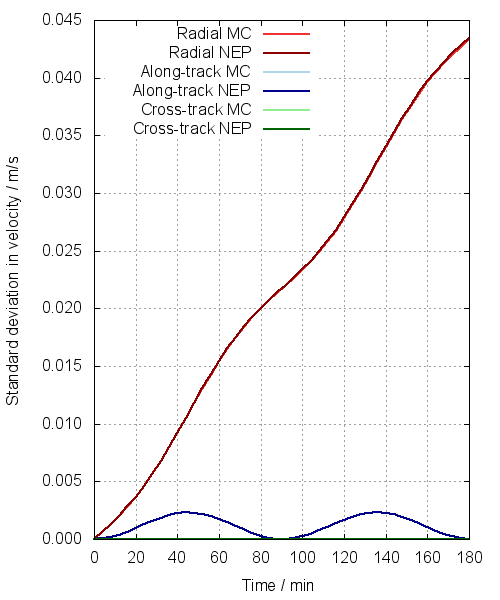
\includegraphics[width=0.4\textwidth]{2B_1_vel.png}}
  \caption{Comparing MC analysis results to \neptune{} covariance matrix propagation using a \SI{60}{\second} integration step size for an initial radial error of \SI{1}{\metre}.\label{fig:val-cov-scen1-01}}
\end{figure}
An error in radial position only leads to a drift in the along-track error as the orbital period is directly affected by the radial component. The latter shows an oscillation with the minimum being at \SI{1}{\metre} and the maximum reaching \SI{3}{\metre} after half an orbit. What can also be observed is that there is no error in the 
orbit normal component as should be expected for a two-body scenario.

It can be seen that there is almost no difference between the numerical propagation in \neptune{} as compared to the results from the \gls{acr:mc} analysis. In \fig{fig:val-cov-scen1-01a} and \fig{fig:val-cov-scen1-01b} the correlation between the along-track position error and the radial velocity error, as well as the correlation between the radial position and along-track velocity component, can be nicely seen. 

The next example in \fig{fig:val-cov-scen1-02} shows the standard deviation evolution for an initial error of \SI{1}{\metre\per\second} for the radial velocity only for the same orbit at \SI{300}{\kilo\metre} altitude and \ang{50;;} inclination. 
\begin{figure}[h!]
  \centering
  \subfigure[Position]{\label{fig:val-cov-scen1-02a} 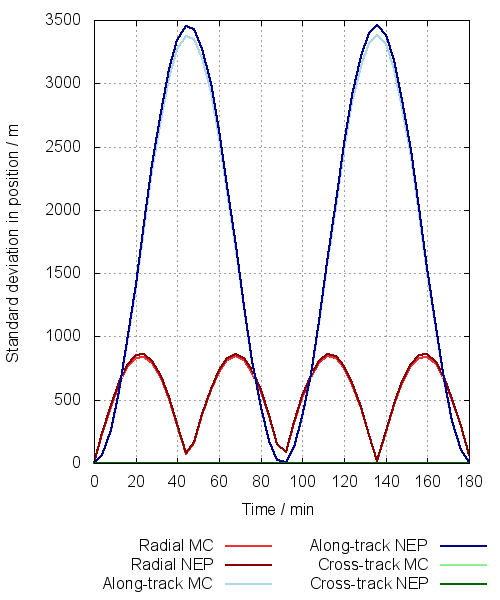
\includegraphics[width=0.4\textwidth]{2B_2_rad.png}}
  \hspace{1cm}
  \subfigure[Velocity]{\label{fig:val-cov-scen1-02b} 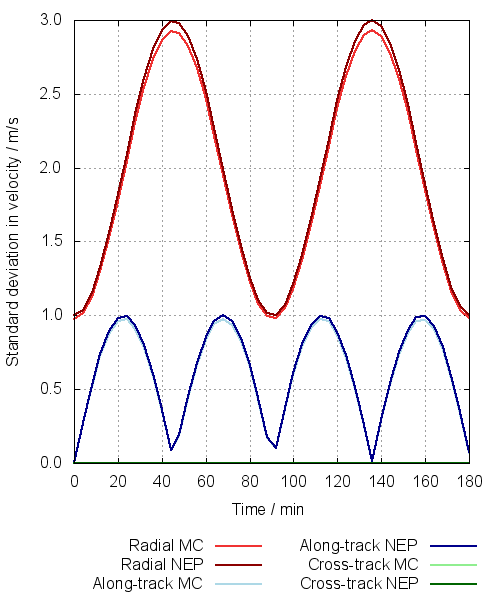
\includegraphics[width=0.4\textwidth]{2B_2_vel.png}}
  \caption{Comparing MC analysis results to \neptune{} covariance matrix propagation using a \SI{60}{\second} integration step size for an initial velocity error of \SI{1}{\metre\per\second}.\label{fig:val-cov-scen1-02}}
\end{figure}
Once again the results show a close alignment between the \gls{acr:mc} approach and \neptune{}'s integration. However, the along-track position error difference at about half an orbit is about \SI{80}{\kilo\metre}, while the error in the radial velocity at the same time is in the order of magnitude of \SI{0.1}{\metre\per\second}. 

This, however, is not indicating an erroneous implementation but is due to the fact that only 500 objects have been used. If the number is increased to 2000 objects, for example, the difference after half an orbit reduces to about \SI{63}{\kilo\metre} in along-track position error and about \SI{0.06}{\metre\per\second} in radial velocity error. 
Increasing the number even further to \num{10000} objects in the \gls{acr:mc} approach leads to a further decrease with the along-track position error difference 
being at about \SI{27}{\kilo\metre} and the radial velocity error difference at \SI{0.025}{\metre\per\second}. Thus, the results obtained by the \gls{acr:mc} analysis are converging towards the 
results from the numerical integration by \neptune{} for an increasing number of objects, which should be expected from the \textit{law of large numbers}.

\paragraph{Scenario 2: Geopotential with order $\gls{sym:geo_n}=2$}

In \sect{sec:propagation-covariance-set-integration-geopotential} the model for the integration of the state error transition matrix under consideration of the 
geopotential is described. This allows to consider, beside the two-body contribution, the evolution of the variances and covariances due to the non-sphericity 
of the Earth within \neptune{}. Especially the Earth's flattening, which is described by the second zonal harmonic coefficient, shows a distinct characteristic 
as is shown in \fig{fig:val-cov-scen2-01}.
\begin{figure}[h!]
  \centering
  \subfigure[Position]{\label{fig:val-cov-scen2-01a} 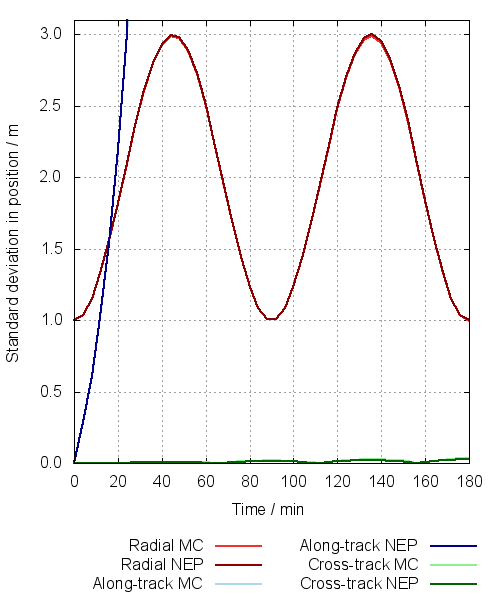
\includegraphics[width=0.4\textwidth]{2BJ2_1_rad.png}}
  \hspace{1cm}
  \subfigure[Velocity]{\label{fig:val-cov-scen2-01b} 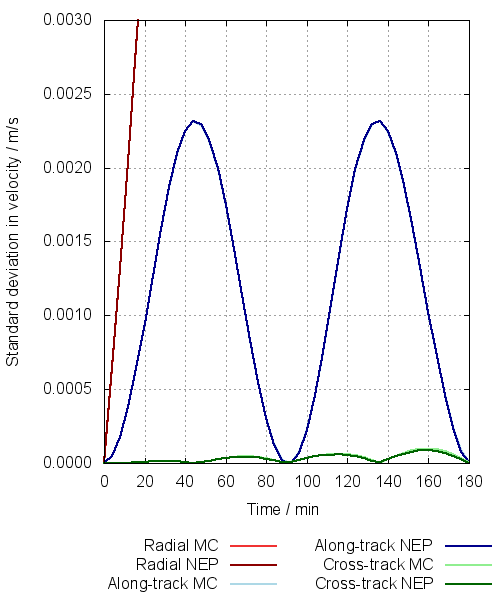
\includegraphics[width=0.4\textwidth]{2BJ2_1_vel.png}}
  \caption{Comparing MC analysis results to \neptune{} covariance matrix propagation using a \SI{60}{\second} integration step size for an initial radial error of \SI{1}{\metre} considering Earth's flattening. \label{fig:val-cov-scen2-01}}
\end{figure}
While the general behaviour in the radial and the along-track component are similar to the one already seen for the two-body case, including Earth's flattening introduces a drift in the orbit normal component. For the velocity normal component, the standard deviation is in the sub-mm/s region after two orbits, while for the position normal the standard deviation is in the centimeter regime. Note, that the simulation again was based on an initial error of \SI{1}{\metre} in the 
radial component.

In \fig{fig:val-cov-scen2-01} the results of \neptune{} closely align with the \gls{acr:mc} analysis. This gives evidence for the correct implementation of the partial derivatives as described in \sect{sec:propagation-covariance-set-integration-geopotential}. One could also look at what happens, if for the \gls{acr:mc} analysis once again the flattened Earth is used, while in \neptune{} the covariance matrix is integrated using the two-body scenario only. The result is shown in \fig{fig:val-cov-scen2-02}.
\begin{figure}[h!]
  \centering
  \subfigure[Position]{\label{fig:val-cov-scen2-02a} 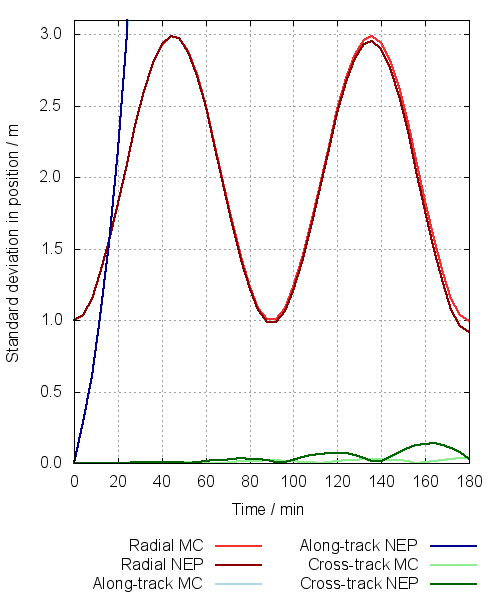
\includegraphics[width=0.4\textwidth]{2BJ2_2_rad.png}}
  \hspace{1cm}
  \subfigure[Velocity]{\label{fig:val-cov-scen2-02b} 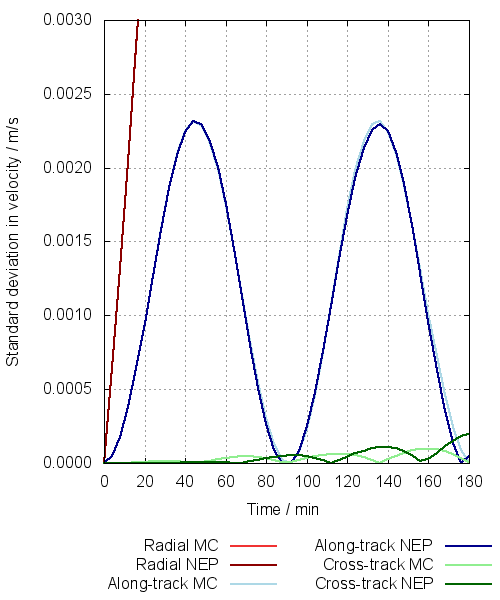
\includegraphics[width=0.4\textwidth]{2BJ2_2_vel.png}}
  \caption{Comparing MC analysis results (incl. Earth's flattening) to \neptune{} covariance matrix propagation using a \SI{60}{\second} integration step size for an initial radial error of \SI{1}{\metre} without Earth's flattening. \label{fig:val-cov-scen2-02}}
\end{figure}
It can be seen that there are significant differences in the radial and the cross-track component for the position error. The normal component even shows a phase shift of half an orbit. One question in this context is why the \neptune{} results for the two-body propagation look different than what was seen in 
\fig{fig:val-cov-scen1-01}. This is due to the fact that the state vector is propagated for a flattened Earth, while the covariance matrix is not. Thus, the state vector is different at each point in time when compared to the two-body propagation, which directly affects the integration of the covariance matrix, as it depends on the current radius vector for each integration step.

\paragraph{Scenario 3: Geopotential with order $\gls{sym:geo_n}>2$}

In \fig{fig:val-cov-scen3-01} the results are shown for a 36 $\times$ 36 geopotential for the same orbit and initial error of \SI{1}{\metre} in the radial position component as already in the previous examples.
\begin{figure}[h!]
  \centering
  \subfigure[Position]{\label{fig:val-cov-scen3-01a} 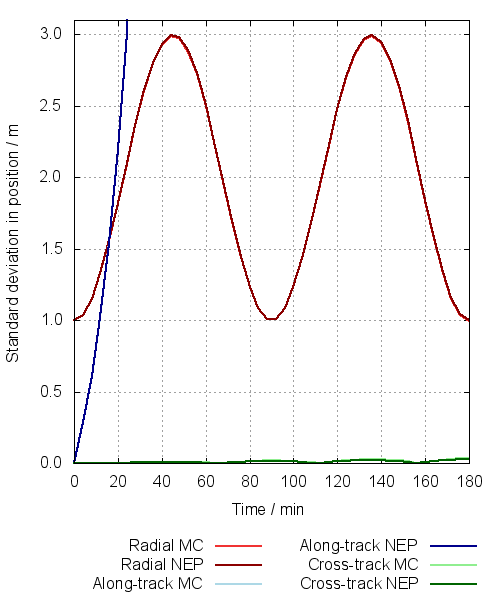
\includegraphics[width=0.4\textwidth]{2BGEOP_1_rad.png}}
  \hspace{1cm}
  \subfigure[Velocity]{\label{fig:val-cov-scen3-01b} 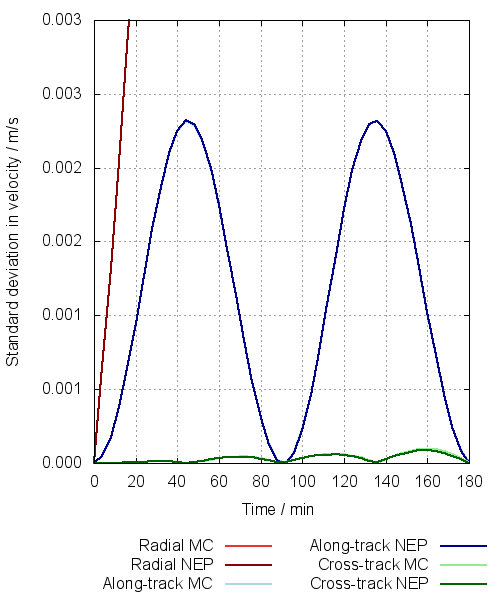
\includegraphics[width=0.4\textwidth]{2BGEOP_1_vel.png}}
  \caption{Comparing MC analysis results to \neptune{} covariance matrix propagation using a \SI{60}{\second} integration step size for an initial radial error of \SI{1}{\metre} considering a 36 $\times$ 36 geopotential. \label{fig:val-cov-scen3-01}}
\end{figure}
The situation looks very similar to the one for a second order geopotential as shown in \fig{fig:val-cov-scen2-01}. The differences are very small so that the 
same simulation was then performed for different orders of the geopotential and then to have a closer look on the normal component in 
\fig{fig:val-cov-scen3-02a} and the radial component in \fig{fig:val-cov-scen3-02b}.
\begin{figure}[h!]
  \centering
  \subfigure[Normal component]{\label{fig:val-cov-scen3-02a} 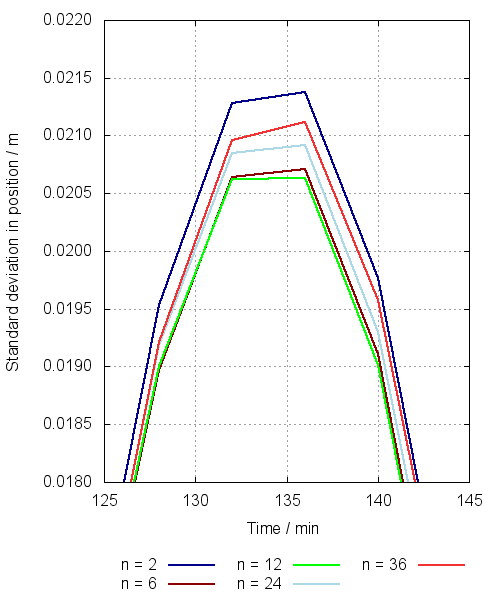
\includegraphics[width=0.4\textwidth]{2BGEOP_2_nor.png}}
  \hspace{1cm}
  \subfigure[Radial component]{\label{fig:val-cov-scen3-02b} 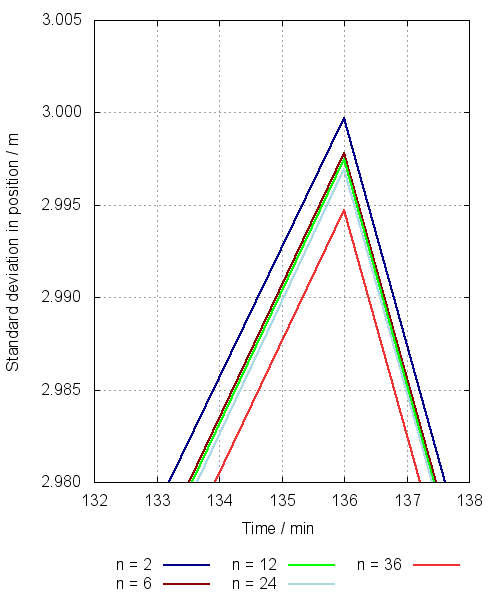
\includegraphics[width=0.4\textwidth]{2BGEOP_2_rad.png}}
  \caption{Sensitivity in covariance matrix propagation for varying order in the geopotential for an initial radial error of \SI{1}{\metre}. \label{fig:val-cov-scen3-02}}
\end{figure}
It can be seen that the error in the standard deviation for the normal component is in the order of magnitude of about \SI{1}{\milli\metre} when comparing a second order 
geopotential to higher orders. This corresponds to about \SI{5}{\percent} variation in this example as the second order geopotential accounts for \SI{2}{\centi\metre} after one and a half orbit. For the radial component the variation by using different order geopotentials is about \SI{5}{\milli\metre}. Note, however, that the number are only an example for that special orbit (\SI{300}{\kilo\metre}, \ang{50;;}) for a short time frame beyond the initial epoch.

In the same context, it is also interesting to look at orbits experiencing resonance effects due to the geopotential. An example shall be given for a \gls{acr:geo}.\todo[Covariance GEO example]{Provide example for GEO resonance effects in covariance matrix propagation.}

\paragraph{Scenario 4: Atmospheric drag}

For orbits experiencing significant drag perturbations it is possible to use additional terms in the variational equations to account for the resulting errors 
in the covariance matrix propagation. An example for a \SI{200}{\kilo\metre}, \ang{54;;} orbit with an initial error of about \SI{3}{\metre} in the along-track position component is shown in \fig{fig:val-cov-scen4-01}, with \neptune integrating only the two-body part for the covariance matrix.
\begin{figure}[h!]
  \centering
  \subfigure[Position]{\label{fig:val-cov-scen4-01a} 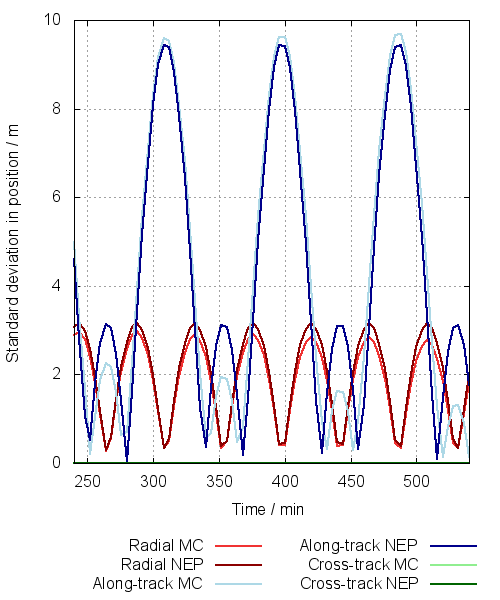
\includegraphics[width=0.4\textwidth]{DRAG_2_rad.png}}
  \hspace{1cm}
  \subfigure[Velocity]{\label{fig:val-cov-scen4-01b} 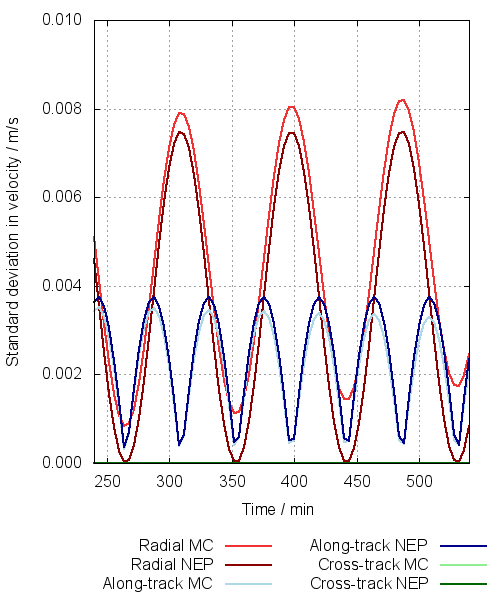
\includegraphics[width=0.4\textwidth]{DRAG_2_vel.png}}
  \caption{Drag perturbed orbit (\SI{200}{\kilo\metre}, \ang{54;;}) with \neptune not accounting for drag in the variational equations for an initial along-track position 
error of \SI{3}{\metre}. \label{fig:val-cov-scen4-01}}
\end{figure}
For the position error in \fig{fig:val-cov-scen4-01a} it can be seen that the error in the along-track component shows a drift of about \SI{10}{\centi\metre} per orbit. The 
increase is not accounted for by \neptune{}. Also, the radial component shows a significant difference after just a few orbits.

A similar behaviour can be observed for the velocity errors in \fig{fig:val-cov-scen4-01b}. The radial component shows a secular increase, while the 
along-track component decreases. Again both trends are not followed by \neptune{}, as expected.\todo[Explain drag deviations]{For the propagation of the covariance matrix, explain deviation with respect to the MC simulation}